\documentclass{beamer}
\usepackage[utf8]{inputenc}
\usetheme{Madrid}
\usecolortheme{default}
\usepackage{amsmath,amssymb,amsfonts,amsthm}
\usepackage{txfonts}
\usepackage{tkz-euclide}
\usepackage{listings}
\usepackage{adjustbox}
\usepackage{array}
\usepackage{tabularx}
\usepackage{gvv}
\usepackage{lmodern}
\usepackage{circuitikz}
\usepackage{tikz}
\usepackage{graphicx}
\setbeamertemplate{page number in head/foot}[totalframenumber]
\usepackage{tcolorbox}
\tcbuselibrary{minted,breakable,xparse,skins}
\definecolor{bg}{gray}{0.95}
\DeclareTCBListing{mintedbox}{O{}m!O{}}{%
  breakable=true,
  listing engine=minted,
  listing only,
  minted language=#2,
  minted style=default,
  minted options={%
    linenos,
    gobble=0,
    breaklines=true,
    breakafter=,,
    fontsize=\small,
    numbersep=8pt,
    #1},
  boxsep=0pt,
  left skip=0pt,
  right skip=0pt,
  left=25pt,
  right=0pt,
  top=3pt,
  bottom=3pt,
  arc=5pt,
  leftrule=0pt,
  rightrule=0pt,
  bottomrule=2pt,
  toprule=2pt,
  colback=bg,
  colframe=orange!70,
  enhanced,
  overlay={%
    \begin{tcbclipinterior}
    \fill[orange!20!white] (frame.south west) rectangle ([xshift=20pt]frame.north west);
    \end{tcbclipinterior}},
  #3,
}
\lstset{
    language=C,
    basicstyle=\ttfamily\small,
    keywordstyle=\color{blue},
    stringstyle=\color{orange},
    commentstyle=\color{green!60!black},
    numbers=left,
    numberstyle=\tiny\color{gray},
    breaklines=true,
    showstringspaces=false,
}
\begin{document}
\title 
{6.2.6}
\date{september 2025}
\author 
{Namaswi-EE25BTECH11060}
\frame{\titlepage}
\begin{frame}{Question}
Find matrix X such that\\
\begin{align}
   X \begin{pmatrix}
        1 & 2 & 3\\
        4 & 5 & 6
    \end{pmatrix}= \begin{pmatrix}
        -7 & -8 & -9 \\ 2 & 4 & 6
    \end{pmatrix}
\end{align}
 \end{frame}
\begin{frame}{Solution}
Form the augmented matrix  
\begin{align}
   \begin{pmatrix}
1 & 4 & | & -7 & -8 & -9 \\
2 & 5 & | & 2 & 4 & 6 \\
3 & 6 & | & 0 & 0 & 0
\end{pmatrix} \\ 
\end{align}
Replace $R_2 \to R_2-2R_1 $ and $R_3 \to R_3-3R_1$
\begin{align}
\begin{pmatrix}
1 & 4 & | & -7 & -8 & -9 \\
0 & -3 & | & 16 & 20 & 27 \\
0 & -6 & | & 21 & 24 & 27
\end{pmatrix} 
\end{align}
\end{frame}
\begin{frame}{Solution}
Replace $R_2 \to \frac{-1}{3}R_2$ and $R_3 \to R_3-2R_2$
\begin{align}
\begin{pmatrix}
1 & 4 & | & -7 & -8 & -9 \\
0 & 1 & | & -16/3 & -20/3 & -9 \\
0 & 0 & | & -11/3 & -16/3 & 9
\end{pmatrix}
\end{align}
Hence,
\begin{align}
    \Vec{X}=\begin{pmatrix}
    1 & 2\\
    -2 &  0
\end{pmatrix}
\end{align}
\end{frame}
\begin{frame}{Solution}
Pseudoinverse verification\\
Let,
\begin{align}
\Vec{A} = \begin{pmatrix}1 & 2 & 3 \\ 4 & 5 & 6\end{pmatrix}\\
\Vec{B} = \begin{pmatrix}-7 & 2 \\ -8 & 4 \\ -9 & 6\end{pmatrix} \\
\Vec{A}^+ &= \Vec{A}^\top (\Vec{A}\Vec{A}^\top)^{-1} \\  
= \begin{pmatrix}
-17/18 & 4/9 \\
-1/9 & 1/9 \\
13/18 & -2/9
\end{pmatrix} 
\end{align}
\end{frame}
\begin{frame}{Solution}
\begin{align}
\Vec{X} &= \Vec{B}\Vec{A}^+ \\  
= \begin{pmatrix}-7 & 2 \\ -8 & 4 \\ -9 & 6\end{pmatrix} 
\begin{pmatrix}-17/18 & 4/9 \\ -1/9 & 1/9 \\ 13/18 & -2/9\end{pmatrix} \\ 
=\begin{pmatrix}1 & 2 \\ -2 & 0\end{pmatrix} 
\end{align} 
\end{frame}
\begin{frame}[fragile]
\frametitle{Python Code}
\begin{lstlisting}
    import numpy as np
import matplotlib.pyplot as plt
from mpl_toolkits.mplot3d import Axes3D

# Create a grid of a and b values
a = np.linspace(-10, 10, 20)
b = np.linspace(-10, 10, 20)
A, B = np.meshgrid(a, b)

# Define the planes
Z1 = -7 - 1*A - 4*B   # a + 4b + z = -7 => z = -7 - a - 4b
Z2 = -8 - 2*A - 5*B   # 2a + 5b + z = -8 => z = -8 - 2a - 5b
Z3 = -9 - 3*A - 6*B   # 3a + 6b + z = -9 => z = -9 - 3a - 6b

\end{lstlisting}
\end{frame}
\begin{frame}[fragile]
\frametitle{Python Code}
\begin{lstlisting}
    # Plot
fig = plt.figure()
ax = fig.add_subplot(111, projection='3d')
ax.plot_surface(A, B, Z1, alpha=0.5, color='red', label='Plane 1')
ax.plot_surface(A, B, Z2, alpha=0.5, color='green', label='Plane 2')
ax.plot_surface(A, B, Z3, alpha=0.5, color='blue', label='Plane 3')

ax.set_xlabel('a')
ax.set_ylabel('b')
ax.set_zlabel('c')
ax.set_title('Graph of 3 Planes')

plt.show()

\end{lstlisting}
\end{frame}
\begin{frame}[fragile]
\frametitle{C Code}
\begin{lstlisting}
    #include <stdio.h>
int main() {
    int i, j, k;
    double a[3][3] = {
        {1, 4, -7},  // a + 4b = -7
        {2, 5, -8},  // 2a + 5b = -8
        {3, 6, -9}   // 3a + 6b = -9
    };
    double factor;
\end{lstlisting}
\end{frame}
\begin{frame}[fragile]
\frametitle{C Code}
\begin{lstlisting}
    // Forward elimination
    for (i = 0; i < 2; i++) { // only first 2 rows, since 2 variables
        for (j = i+1; j < 3; j++) {
            if(a[i][i] != 0){
                factor = a[j][i] / a[i][i];
                for (k = i; k < 3; k++) {
                    a[j][k] -= factor * a[i][k];
                }
            }
        }
    }
\end{lstlisting}
\end{frame}
\begin{frame}[fragile]
\frametitle{C Code}
\begin{lstlisting}
    // Back substitution
    double b_val, a_val;
    if(a[1][1] != 0){
        b_val = a[1][2] / a[1][1];
        a_val = (a[0][2] - 4*b_val) / 1;
        printf("Solution: a = %.2lf, b = %.2lf\n", a_val, b_val);
    } else {
        printf("No unique solution exists.\n");
    }
    return 0;
}
\end{lstlisting}
\end{frame}
\begin{frame}[fragile]
\frametitle{C and Python Code}
\begin{lstlisting}
   import ctypes

# Load shared library
lib = ctypes.CDLL('./libsolver.so')

# Prepare variables
a = ctypes.c_double()
b = ctypes.c_double()
status = ctypes.c_int()
 
\end{lstlisting}
\end{frame}
\begin{frame}[fragile]
\frametitle{C and Python Code}
\begin{lstlisting}
    # Call C function
lib.solve_system(ctypes.byref(a), ctypes.byref(b), ctypes.byref(status))

# Check result
if status.value == 1:
    print(f"Solution from C: a = {a.value}, b = {b.value}")
else:
    print("No unique solution exists.")
\end{lstlisting}
\end{frame}
\begin{frame}{Plot}
    \centering
    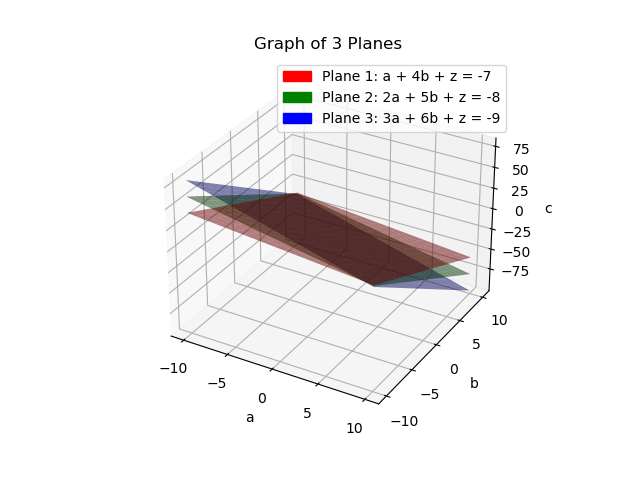
\includegraphics[width=\columnwidth, height=0.8\textheight, keepaspectratio]{Figure_13.png}     
\end{frame}
\end{document}
